%% ===================================================================
\section{Experiments}
\label{sec:experiments}
%% ===================================================================

Our evaluation follows the three capabilities of \cref{sec:framework}. \AEGIS \emph{audits} (\cref{sec:audit}): one analytic query matches iterative attackers and its $S_c$ ranking transfers to discrete edge removal across architectures. It \emph{certifies} (\cref{sec:certify}): \AEGIS-Conformal coverage holds at the nominal level under the very attack it certifies, where randomized smoothing is vacuous. It \emph{defends} (\cref{sec:defense}): a $\sigma_1(S_c)$ penalty buys certified robustness. A deployed fraud detector (\cref{sec:fraud_case}) closes the loop on real data.

\textbf{Setup.} We evaluate \AEGIS on 6 datasets across 4 domains with 10 seeds each (PyTorch~\cite{paszke2019pytorch}); $\pm$ are seed standard deviations. IGNN~\cite{gu2020implicit} uses $F(Z){=}\mathrm{ReLU}(\Ahat ZW^\top{+}U(X))$, $W\in\R^{64\times64}$ spectral-normalised~\cite{miyato2018spectral}, Adam (lr $0.01$). Datasets: Cora, Citeseer, Pubmed~\cite{sen2008collective}, Amazon Photo~\cite{shchur2018pitfalls}, WikiCS~\cite{mernyei2020wiki}, Amazon Fraud~\cite{dou2020enhancing}; baselines: smoothing (Gaussian $\sigma{=}0.01$), Mettack, GR-BCD/PR-BCD~\cite{geisler2021robustness}. All seven architectures appear only in \cref{fig:tau_heatmap} and \cref{tab:explicit}; the rest use IGNN. Full tables, ablations, and timing are in \cref{app:experiments}; reproducibility in \cref{app:repro}.

%% ----------------------------- AUDIT -----------------------------
\subsection{Audit: One Query Finds the Worst Attack}
\label{sec:audit}\label{sec:adaptive}\label{sec:certificates}\label{sec:cross_domain}

Two prerequisites must hold: the trained models sit in the contractive regime, and \AEGIS's perturbations beat chance. \Cref{tab:cross_domain} confirms both, verifying (A3) on every benchmark ($\kappa{<}1$) and reporting per-dataset $\ecrit$ alongside a $3.2$--$4.1\times$ attack advantage over random. Unless stated otherwise, IGNN experiments run on 50-node BFS ego-subgraphs centred on the highest-degree node and report \emph{local} vulnerability, while graph-level assessment uses the matrix-free pipeline (\cref{app:phase_scal}); all bounds use $\kappa{=}\norm{J_z}_2$.

\begin{table}[t]
\centering
\caption{Per-dataset IGNN characterisation (10 seeds). $\kappa{=}\norm{J_z}_2$ verifies (A3); $\ecrit{=}(1{-}\kappa)/\norm{W}_2$ is the local critical budget. AtkAdv: \AEGIS/random damage. Cov\%: subgraph nodes certified first-order-safe at $\varepsilon{=}0.05$ ($r_v{>}0.05$).}
\label{tab:cross_domain}
\footnotesize
\setlength{\tabcolsep}{4pt}
\begin{tabular*}{\columnwidth}{@{\extracolsep{\fill}}l r r r r r@{}}
\toprule
Dataset & Test Acc & $\kappa$ & $\ecrit$ & AtkAdv & Cov\% \\
\midrule
Cora     & $\ms{77.5}{1.7}$ & $\ms{.33}{.14}$ & $\ms{.66}{.15}$ & $\ms{3.6}{.6}$ & $\ms{83}{10}$ \\
Citeseer & $\ms{66.0}{0.7}$ & $\ms{.59}{.02}$ & $\ms{.41}{.02}$ & $\ms{4.1}{.5}$ & $\ms{94}{5}$ \\
Pubmed   & $\ms{78.9}{0.7}$ & $\ms{.41}{.11}$ & $\ms{.59}{.11}$ & $\ms{3.2}{.4}$ & $\ms{76}{18}$ \\
Amazon   & $\ms{94.8}{0.3}$ & $\ms{.14}{.02}$ & $\ms{.86}{.02}$ & $\ms{3.8}{.2}$ & $\ms{86}{8}$ \\
WikiCS   & $\ms{77.9}{0.4}$ & $\ms{.34}{.04}$ & $\ms{.66}{.04}$ & $\ms{3.8}{.4}$ & $\ms{78}{4}$ \\
\bottomrule
\end{tabular*}
\end{table}

\textbf{One-query attack.} \AEGIS's attack is analytic and costs a single query, not an optimisation loop: by construction the SVD direction maximises the first-order equilibrium shift (\cref{prop:attack}). Three findings show that this single query reflects the model rather than a gradient artifact. First, a transfer direction from a \emph{separately trained} surrogate (zero shared gradients) recovers $99\%$ of the one-query damage ($\cos{=}0.99$), against $44{\pm}4\%$ for a $512$-query black-box search. Second, per query the attack delivers $\mathbf{74}$--$\mathbf{156\times}$ the \emph{equilibrium-shift} damage of a $50$-step PGD~\cite{madry2018towards} (\cref{tab:attack_full}); classification-loss PGD inflicts $15$--$70\%$ less at $50\times$ the cost, and GR-BCD pulls ahead only at the larger budgets it is designed for (\cref{app:baselines}). Third, per-edge finite differences reproduce the $S_c$ column-norm ranking ($\tau{=}0.999$), and iterative recomputation closes at most $3$\,pp of the static-versus-greedy gap at $k{\times}$ the compute, so the static ranking stands as the headline.

\begin{table}[t]
\centering
\caption{One-query audit vs.\ iterative attackers: equilibrium damage at $\varepsilon{=}0.10$ (IGNN, 50-node subgraph, 10 seeds). Cls-PGD: classification-loss PGD; Shift-PGD: IFT-gradient PGD (solver validation, not an independent baseline).}
\label{tab:attack_full}
\small
\setlength{\tabcolsep}{4pt}
\begin{tabular*}{\columnwidth}{@{\extracolsep{\fill}}l rrrr@{}}
\toprule
Dataset & \AEGIS & Cls-PGD & Shift-PGD & Random \\
\midrule
Cora     & $\ms{3.70}{.79}$ & $\ms{2.51}{.48}$ & $\ms{3.05}{.70}$ & $\ms{0.97}{.25}$ \\
Citeseer & $\ms{4.63}{.71}$ & $\ms{2.97}{.42}$ & $\ms{3.35}{.57}$ & $\ms{1.01}{.15}$ \\
WikiCS   & $\ms{2.10}{.22}$ & $\ms{0.67}{.11}$ & $\ms{1.93}{.20}$ & $\ms{0.53}{.09}$ \\
\bottomrule
\end{tabular*}
\end{table}

\AEGIS also beats degree-proportional, edge-betweenness, and spectral rankings at $\varepsilon{=}0.01$ ($+6$--$148\%$ AtkAdv), and inflicts $3$--$10\times$ more equilibrium damage than Mettack~\cite{zugner2019adversarial} in the early-warning regime ($\mathbf{149/150}$ paired wins, $p{<}10^{-43}$). The discrete-removal curves against a label-aware Greedy attacker appear in \cref{fig:greedy_topk}, with GR-BCD/PR-BCD detail in \cref{app:baselines}. As a check on the linearisation, the first-order shift bounds agree with the actual shifts to within $1\%$ at small budgets, loosening to ${\leq}39\%$ on citation graphs by $\varepsilon{=}0.20$.

\textbf{Breach rates.} Every breached node satisfies $\varepsilon > r_v$ across all datasets and budgets, validating $r_v$ as a reliable first-order screen (\cref{sec:certify}). \Cref{fig:breach} reports prediction-flip fractions vs.\ $\varepsilon$ ($95\%$ CI bands): Citeseer and WikiCS stay below $2\%$ throughout; Cora reaches $7.6\%$ at $\varepsilon{=}0.20$; Pubmed is the right-skewed outlier (mean $10.3\%$ at $\varepsilon{=}0.10$, $27.4\%$ at $\varepsilon{=}0.20$).

\begin{figure*}[t]
\centering
\begin{minipage}[t]{0.33\textwidth}
\centering
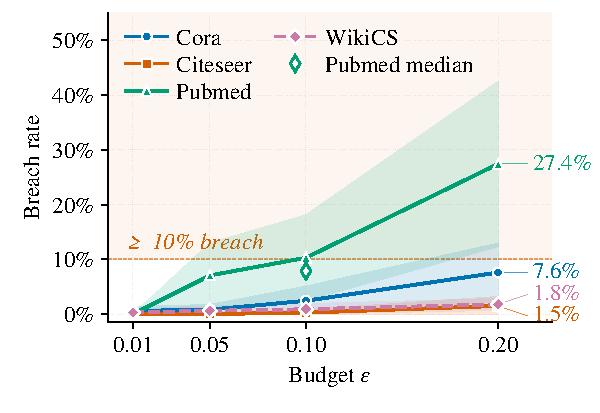
\includegraphics[width=\linewidth]{figures/fig_breach_rate.pdf}
\caption{Breach rate (\% of nodes flipped under $S_c$-optimal perturbation) vs.\ $\varepsilon$ (10 seeds; mean, $95\%$ CI bands).}
\label{fig:breach}
\end{minipage}\hfill
\begin{minipage}[t]{0.655\textwidth}
\centering
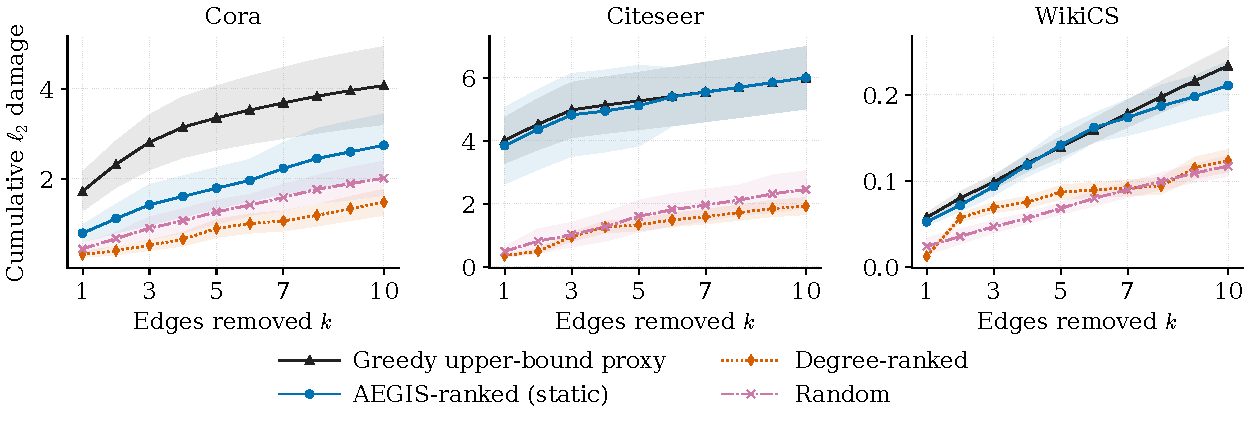
\includegraphics[width=\linewidth]{figures/fig_greedy_curves.pdf}
\caption{Cumulative damage from sequential discrete edge removal vs.\ $k$ (IGNN, 50-node subgraph, 10 seeds). \AEGIS \emph{matches} the label-aware Greedy attacker on Citeseer/WikiCS and recovers $\mathbf{54}$--$\mathbf{67\%}$ of its Cora damage at $k{=}5$--$10$ with no discrete-label access; degree-ranking stays below random.}
\label{fig:greedy_topk}
\end{minipage}
\end{figure*}

\textbf{Continuous-to-discrete transfer.}\label{sec:explicit_extension} The construction is not tied to implicit models. For $K$-layer explicit GNNs (GCN, SAGE, GIN, APPNP, GAT$^\dagger$~\cite{kipf2017semi,hamilton2017inductive,xu2019how,klicpera2019predict,velickovic2018graph}) we form $S_K{=}\partial \mathrm{vec}(Z_K)/\partial \mathrm{vec}(A)$ by finite differences and build $S_c$ exactly as before (\cref{prop:explicit}); only the IGNN additionally carries the boundary of \cref{thm:phase_transition}. The question that matters in practice is whether the continuous $S_c$ ranking predicts the discrete, brute-force N-1 removal order. Ranking edges by the edge-weighted score $A_{ij}v_{ij}$ of \cref{prop:transfer}, \cref{fig:tau_heatmap} reports the Kendall $\tau$ over 6 datasets and 7 architectures (390 runs): every one of the $\mathbf{39/39}$ cells is positive, with median $\tau{=}\mathbf{+0.99}$ ($p{<}10^{-5}$), against $34/39$ for the unweighted score. The agreement even survives leaving the contractive regime: on full-graph Amazon Photo ($N{=}7{,}650$, $\kappa{\approx}1.00$) it reaches $\tau\!=\!\mathbf{+0.996\!\pm\!0.002}$. Per-architecture detail, the phase-transition and scalability sweeps (the matrix-free path reaching $N{=}7{,}650$), and the ablations are in \cref{app:explicit,app:phase_scal,app:ablations}; the ablations show vulnerability to be \emph{delocalized}, so $S_c$ localises risk for triage rather than removing it.

\begin{figure}[t]
\centering
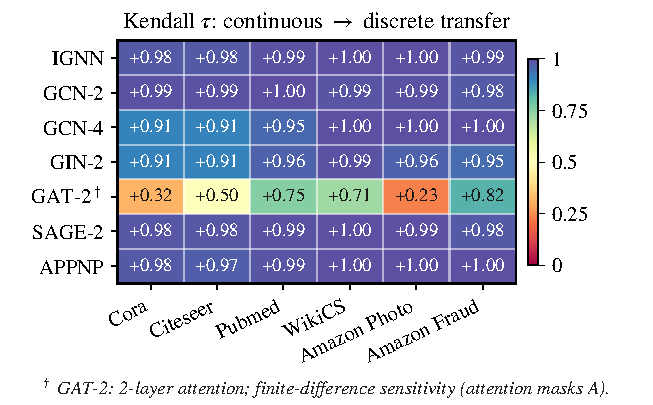
\includegraphics[width=\columnwidth]{figures/fig_tau_heatmap.pdf}
\caption{Continuous-to-discrete transfer $\tau$ (10-seed means; per-cell sd $0.0003$--$0.041$). Cross-hatch: GPU OOM. GAT-2$^\dagger$ is lower under weighting (it transfers better unweighted; see \cref{app:explicit}).}
\label{fig:tau_heatmap}
\end{figure}

%% ----------------------------- CERTIFY -----------------------------
\subsection{Certify: Distribution-Free Coverage}
\label{sec:certify}

The certificate of \cref{sec:conformal} holds empirically. \Cref{tab:conformal} reports coverage over 10 seeds and four datasets. The crucial quantity is the \emph{gate}, the coverage retained under the worst-case \AEGIS attack at magnitude $\varepsilon$: it sits at the nominal $1{-}\alpha{=}0.90$ at $\varepsilon{=}0.01$ on every dataset and turns conservative ($0.94$--$1.00$) at $\varepsilon{=}0.05$. The sets stay informative throughout, running ${\sim}1.0$--$3.5$ labels and tightening exactly where the deterministic radius is thin, all at zero Monte-Carlo samples. Two conditions are stated plainly: exchangeability on a single transductive graph is an assumption for which the empirical gate is the evidence, and $S_c$ is formed densely at $N{=}200$, leaving a matrix-free conformal pass to future work.

\begin{table}[t]\centering\footnotesize\setlength{\tabcolsep}{4pt}
\caption{\AEGIS-Conformal coverage (10 seeds; Cora, Citeseer, Pubmed, WikiCS; $\alpha{=}0.1$, target $0.90$). Each $\varepsilon$ block reports clean coverage\,/\,mean set size, then the bold \textbf{gate} (coverage under the worst-case attack at $\varepsilon$). Classes: 7/6/3/10 resp.; std over seeds ${\leq}0.07$. Sets ${<}1$ reflect occasional empty (abstaining) sets under TPS.}
\label{tab:conformal}
\begin{tabular*}{\columnwidth}{@{\extracolsep{\fill}}ll cc cc@{}}
\toprule
Data & score & \multicolumn{2}{c}{$\varepsilon{=}0.01$} & \multicolumn{2}{c}{$\varepsilon{=}0.05$} \\
\cmidrule(lr){3-4}\cmidrule(lr){5-6}
Cora     & APS & 0.90 / 1.37 & \textbf{0.90} & 0.89 / 1.06 & \textbf{0.98} \\
         & TPS & 0.88 / 0.95 & \textbf{0.90} & 0.89 / 0.99 & \textbf{0.98} \\
\addlinespace
Citeseer & APS & 0.92 / 1.50 & \textbf{0.92} & 0.92 / 1.35 & \textbf{0.97} \\
         & TPS & 0.91 / 1.20 & \textbf{0.92} & 0.92 / 1.26 & \textbf{0.96} \\
\addlinespace
Pubmed   & APS & 0.91 / 1.42 & \textbf{0.95} & 0.92 / 1.52 & \textbf{1.00} \\
         & TPS & 0.90 / 1.15 & \textbf{0.92} & 0.90 / 1.15 & \textbf{0.98} \\
\addlinespace
WikiCS   & APS & 0.92 / 3.70 & \textbf{0.94} & 0.93 / 3.62 & \textbf{0.95} \\
         & TPS & 0.93 / 3.52 & \textbf{0.94} & 0.93 / 3.52 & \textbf{0.95} \\
\bottomrule
\end{tabular*}
\end{table}

\Cref{tab:smoothing} pits \AEGIS-Conformal against randomized smoothing: on the matched Frobenius ball smoothing is \emph{vacuous} (full label set, zero certified nodes); only on a strictly larger per-coordinate ball does it certify, and then at $\mathbf{23{,}000}$--$\mathbf{57{,}000\times}$ the cost of the zero-sample $S_c$ bound (\cref{app:smoothing}).

\begin{table}[t]\centering\footnotesize\setlength{\tabcolsep}{2pt}
\caption{\AEGIS-Conformal vs.\ randomized smoothing (Cora, $n{=}200$, 10 seeds, $\alpha{=}0.1$, APS). \textbf{frob}: matched Frobenius ball ($\sigma{=}\varepsilon/\sqrt{2|E|}$); \textbf{per\_edge}: larger per-coordinate ball ($\sigma{=}\varepsilon$), favorable to smoothing. cert: fraction certified; wall-clock at $M{=}10^4$ samples (\AEGIS-Conformal is zero-sample).}
\label{tab:smoothing}
\begin{tabular*}{\columnwidth}{@{\extracolsep{\fill}}llccccc@{}}
\toprule
method & match & $\varepsilon$ & cov & set & cert & wall@$10^4$ \\
\midrule
\AEGIS-Conformal & --       & 0.01 & 0.90 & 1.36 & --   & \textbf{${\sim}1$\,s} \\
RandSmoothing    & frob     & 0.01 & 1.00 & 7.00 & 0.00 & 7{,}600\,s \\
RandSmoothing    & per\_edge& 0.01 & 0.95 & 1.26 & 0.96 & 15{,}000\,s \\
\midrule
\AEGIS-Conformal & --       & 0.05 & 0.90 & 1.05 & --   & \textbf{${\sim}1$\,s} \\
RandSmoothing    & frob     & 0.05 & 1.00 & 7.00 & 0.00 & 10{,}900\,s \\
RandSmoothing    & per\_edge& 0.05 & 0.99 & 2.39 & 0.77 & 36{,}300\,s \\
\bottomrule
\end{tabular*}
\end{table}

%% ----------------------------- DEFEND -----------------------------
\subsection{Defend: A $\sigma_1(S_c)$ Robustness Knob}
\label{sec:defense}

The operator that finds the worst attack also tunes the defense. Penalizing $\sigma_1(S_c)$ during training drives the dominant sensitivity down, and with it the worst-case attack damage falls while the certified fraction rises (\cref{tab:defense}). At the operating point $\lambda{=}3{\times}10^{-4}$ this cuts $\sigma_1$ by ${\sim}10\times$ ($\ms{319}{59}\!\to\!\ms{32.6}{1.7}$) and lifts the certified fraction to $0.82{\pm}0.03$, at a cost of roughly 4 accuracy points. The gain is genuinely \emph{certified} rather than empirical: at $\varepsilon{\leq}0.1$ few nodes flip for either model (the delocalized vulnerability noted above), so the penalty buys a larger certified margin, not better small-budget accuracy. Attack and defense thus couple through the one operator: across 10 seeds the margin-controlled attack magnitude and the certified radius are anticorrelated ($-0.65{\pm}0.12$, negative in $\mathbf{10/10}$ seeds, $p{\approx}10^{-160}$).

\begin{table}[t]
\centering
\caption{The $\sigma_1(S_c)$ penalty trades clean accuracy for certified robustness (Cora, $c{=}0.9$ IGNN, 10 seeds). Cert.\ frac peaks at $\lambda{=}3{\times}10^{-3}$ before margin collapse.}
\label{tab:defense}
\footnotesize
\setlength{\tabcolsep}{4pt}
\begin{tabular*}{\columnwidth}{@{\extracolsep{\fill}}r r r r r@{}}
\toprule
$\lambda$ & Acc & $\sigma_1(S_c)$ & Cert.\ frac & Attack dmg \\
\midrule
$0$               & $\ms{.781}{.018}$ & $\ms{319}{59}$  & $\ms{.40}{.08}$ & $\ms{27.8}{6.3}$ \\
$3{\times}10^{-4}$ & $\ms{.739}{.008}$ & $\ms{32.6}{1.7}$ & $\ms{.82}{.03}$ & $\ms{3.1}{0.2}$ \\
$1{\times}10^{-3}$ & $\ms{.690}{.007}$ & $\ms{10.7}{0.6}$ & $\ms{.89}{.02}$ & $\ms{1.1}{0.1}$ \\
$3{\times}10^{-3}$ & $\ms{.619}{.006}$ & $\ms{3.9}{0.2}$  & $\ms{.92}{.02}$ & $\ms{0.4}{0.0}$ \\
$1{\times}10^{-2}$ & $\ms{.564}{.006}$ & $\ms{0.8}{0.1}$  & $\ms{.86}{.04}$ & $\ms{0.1}{0.0}$ \\
\bottomrule
\end{tabular*}
\end{table}
